\documentclass{article}
\usepackage{graphicx} % Required for inserting images
\usepackage{biblatex} % Imports biblatex package
\addbibresource{references.bib}
\usepackage{changepage}
\usepackage{parskip}
\usepackage{subfig}
\usepackage{multirow}

\title{Interpretable Deepfake Voice Detection: A Hybrid Deep-Learning Model and Explanation Evaluation}
\date{2024-10-01} 
\author{Jacob LaRock\\1667321}
\linespread{1.5}

\def\Institute{Universität Siegen}
\def\KindOfWork{Bachelorarbeit}
\def\Studiengang{Wirtschaftsinformatik}
\def\Fakultaet{Fakultät III: Wirtschaftswissenschaften, Wirtschaftsinformatik und Wirtschaftsrecht}
 
\def\Title{Interpretable Deepfake Voice Detection: A Hybrid Deep-Learning Model and Explanation Evaluation}
\def\Subtitle{}
 
\def\student{Jacob LaRock}
\def\studentno{1667321}
\def\place{Siegen}
\def\Date{17.03.2025} 
\def\semester{6}
 
\def\erstpruefer{Univ.-Prof. Dr. Gunnar Stevens}
\def\erstprueferMail{Gunnar.Stevens@uni-siegen.de}
\def\zweitpruefer{Univ.-Prof. Dr. Volker Wulf}
\def\zweitprueferMail{Volker.Wulf@uni-siegen.de}

\makeatletter
\newcommand\notsotiny{\@setfontsize\notsotiny\@vipt\@viipt}
\makeatother

\begin{document}
	\begin{titlepage}
        \begin{minipage}{0.9\linewidth}
			\centering
			
\includegraphics [width=0.35\textwidth]{images/LogoSiegen}
        \end{minipage}

		\vspace{2cm}

		\centering

		{\Large\bfseries \Title\par}
		{\large\bfseries \Subtitle\par}
		\vspace{1.5cm}

		{\large \textbf{\KindOfWork}\par}

		\vspace{1cm}

		{\normalsize im Studiengang \\
			\Studiengang \ im \semester. Semester \\
		}
		\vspace{0.5cm}
		{\normalsize vorgelegt von}
		\vspace{0.5cm}

		{\normalsize \textbf{\student} \\
			Matr.-Nr.: \studentno  \\}
		{am \normalsize \Date\par}

		\vspace{0.5cm}

		{\Institute} \par
		{\Fakultaet}\par

		\vspace{0.5cm}

    {\begin{table}[ht]
			\centering\small
			\begin{tabular}{lll}
				{Erstprüfer:} & \erstpruefer & \erstprueferMail \\
				{Zweitprüfer:} & \zweitpruefer & \zweitprueferMail \\
			\end{tabular}
		\end{table}}     
		\vfill
	\end{titlepage}
    \newpage
\section{Abstract}
\sloppy
With the unprecedented advancement of Generative Artificial Intelligence (GenAI), the threat of voice scams using synthetic voices has become a serious concern across various sectors. Recent efforts have focused on identifying fake voices through handcrafted features, deep learning models, and hybrid approaches. However, most existing methods lack explainability, rendering their predictions non-transparent to users. This paper proposes a novel, interpretable, and transparent method for fake voice identification by introducing a hybrid deep learning model that leverages multiple extracted features. The hybrid model consists of two main components: the first component addresses heterogeneous feature spaces by employing deep convolutional sub-models tailored to individual features, while the second component, the terminus model, utilizes the concatenated representations from the final layers of each sub-model as input. The terminus model follows a typical multi-layer perceptron architecture, enabling effective integration and classification of the diverse feature representations. To enhance interpretability, we decompose the model’s decisions using Local Interpretable Model-agnostic Explanations (LIME), taking advantage of the identical feature representation before the concatenation layers to address challenges related to multidimensional feature representations. To evaluate the features and assess the quality of the generated explanations, we propose two metrics: importance and trust. Extensive experiments are conducted on the In-the-Wild dataset, which is designed to test the generalization capability of synthetic audio detection methods. The experimental results demonstrate that our approach achieves performance comparable to benchmark methods. Furthermore, the results based on our proposed metrics conclude that certain perceptible features demonstrate promise for generating explanations that are meaningful to general users. For reproducibility, the source code for these experiments is available in the following repository: \url{https://github.com/jacoblarock/fake_voices_xai}

\section{Introduction}
Since the use of generative methods for creating synthetic voices has become more widespread, the need for reliable and usable detection methods to protect the security of individuals and businesses has grown. In particular, the rise of deepfake technology has raised concerns about its potential misuse in areas such as politics, entertainment, and national security. For instance, malicious actors could exploit this technology to create fake audio recordings that appear to be genuine statements made by public figures or to fabricate recordings of events that never occurred. Such misuse could have significant consequences, including the spread of misinformation, defamation of individuals, and the escalation of political tensions \cite{veerasamy_rising_2022,albahar_deepfakes_2005}.

There has been considerable attention on identifying audio deepfakes using classical and sophisticated deep learning models~\cite{wang2020deepsonar,becker2024audiomnist,muller_does_2022,yang_robust_2024,wang_asvspoof_2020}. Methods for fake voice identification can be broadly categorized into two classes: methods with handcrafted feature extraction and methods with end-to-end deepfake detectors~\cite{dixit2023review,li2025survey}. In the former, detection approaches first extract various features from the voices. These high-dimensional feature values are then passed through complex deep learning models to determine whether the voice is real or synthesized (i.e., fake). End-to-end fake voice identification methods generally optimize the feature extraction process and classification task jointly. Both methods, however, have shown promise in the field to produce reliable results.

The field of Explainable AI (XAI) shows promise for producing useful and interpretable results from such models. Explainable AI refers to the ability of artificial intelligence systems, such as machine learning models and neural networks, to provide understandable and interpretable explanations for their decisions or predictions~\cite{hind_explaining_2019}. This means that XAI systems can articulate why they made a particular decision, what factors influenced it, and how confident they are in their conclusion \cite{hind_explaining_2019}. Although the application of XAI has increased exponentially in other domains, including health informatics, natural language processing, and image processing, its use in fake voice identification is less frequent. One probable reason is that voice consists of signals, and explanations leveraging signals might pose more challenges in the presentation of results to end users than in other domains. For example, explanations highlighting objects in object identification or relevant words in text sentiment classification can make sense to users.

For the detection of audio deepfakes, the application of XAI methods could mean that the model can justify its classification with feature-based evidence, allowing for verification of the result by the end user. Much of the existing research, further discussed in section \ref{sec:related}, focuses on producing models with the best possible benchmarks against datasets of samples, without considering whether the results can be usefully interpreted. Existing explorations into making audio deepfake detection explainable have produced results that often require significant background knowledge to interpret meaningfully. Aside from this, explainability in the area of audio deepfake detection remains an open challenge \cite{cuccovillo_open_2022}, one even promoted by regulatory bodies such as the European Union with the so-called "right to explain"~\cite{goodman_european_2017}.

One popular method to detect synthetic voices is to use images consisting of Mel-spectrograms derived from voice signals. Deep learning classifiers then utilize these generated images to predict whether the voice is original or fake. However, applying XAI to such methods is not meaningful because explanations considering pixels as elements would not be understandable to general users. Such explanations can help AI practitioners understand the problem and modify models to achieve higher accuracy. An alternative solution for explaining predictions in fake voice identification is a feature extraction-based approach, making use of features that can be perceived by the average ear. In this case, predictions can be explained using understandable features.

In this work, we introduce a hybrid deep learning model leveraging perceptible features extracted from voice signals. The dimensions of each perceptible feature are not the same. Therefore, our hybrid model consists of a component sub-model for each input feature to address the problem of varying dimensionality of the extracted features without the drawbacks of costly transformations in the pre-processing phase. The concatenation of the sub-models' outputs is followed by a terminus model. The terminus model, which uses the concatenated outputs of the individual sub-models as inputs, distills its inputs into a singular output using a classic multi-layer perceptron architecture, allowing for an effective combination of the features into a final classification result.

In order to maximize the potential of our method, we make the distinction between two categories of extractable features, perceptible and imperceptible, with imperceptible features being unlikely to be heard by the human ear and thus likely ill-suited for an understandable explanation. Examples of imperceptible features would be spectrographic representations of the audio or cepstral coefficients, which are widely used in other works, as discussed in Section \ref{sec:related_imperceptible}. Perceptible features are features that can be perceived by the human ear, such as jitter, shimmer or pitch fluctuation, which have a wide range of uses even outside of audio classification, such as in disease diagnosis \cite{chaiwongyen_deepfake-speech_2023}.

To introduce explainability into our method, we generate explanations using the output of each sub-model before the concatenation layers and then apply Local Interpretable Model-agnostic Explanations (LIME) \cite{ribeiro_why_2016} on the terminus model. This allows us to assess the impact of each input feature on the final result through local explanations. Due to the independence of the sub-models, the importance of their outputs directly correlates with the importance of their inputs for the end classification made by the terminus model.

We then faced the problem of assessing our explanations, specifically evaluating the impact of the input features on the average local explanation to determine the usefulness of our chosen features for providing understandable explanations of our model's classifications. Other methods for assessing the global impact of features exist, such as SHAP (SHapley Additive exPlanations) \cite{lundberg2017unified}. However, because such methods use principles different from those of LIME for assessing the impact of features on a global scale, they do not necessarily represent the presence of the features within the average explanation generated by LIME. Due to this, as well as the fact that existing research lacks methods of aggregate evaluation of many LIME explanations, we therefore introduce two metrics: \textit{trust} and \textit{importance}. These metrics allow for an aggregate evaluation of a large number of generated LIME explanations on a per-feature basis, enabling us to assess the usefulness of the features within a given feature set for producing useful and understandable explanations.

We conducted a wide range of experiments to evaluate the performance of our hybrid audio deepfake detection approach on the \textit{In-The-Wild} dataset. The experimental results demonstrate that our model performs effectively compared to state-of-the-art methods. The evaluation of the generated explanations using our proposed metrics also identifies which features have the highest impact on the model's overall predictions. The contributions of this paper are twofold:
\begin{itemize}
\item We propose an interpretable hybrid deep learning model to identify synthetic voices using perceptible features.
\item We propose two metrics in order to perform aggregate evaluations of many explanations from our LIME-based method, in order to assess how useful the average explanation is.
\end{itemize}

This paper is divided into the following sections: Section \ref{sec:related} presents the most relevant research conducted in this field. Section \ref{sec:method} describes our proposed hybrid deep learning model and the evaluation metrics introduced to judge the generated explanations. The next section, section \ref{sec:experimental_results} presents the experimental setup, results, and performance comparisons. Section \ref{sec:discussion} discusses the implications of the results and limitations of our method. Finally, the last section concludes the paper with possible future work.

\section{Related Work} \label{sec:related}

The detection of fake voices has received significant attention in recent years. This section presents relevant research that utilizes hand-crafted features, both perceptible and imperceptible. Additionally, we highlight efforts within the research community to enhance the explainability of fake voice identification methods.

\subsection{Synthetic Voice Detection with Imperceptible Features} \label{sec:related_imperceptible}

The most common approach in this domain involves using either learned or hand-crafted imperceptible features. Examples include spectrographic features such as mel-spectrograms and their hand-crafted derivatives, such as mel-frequency cepstral coefficients (MFCCs), both of which are widely used due to their effectiveness.

Anagha et al.~\cite{anagha_audio_2023} utilized mel-spectrograms in combination with a convolutional neural network (CNN)-based architecture, achieving strong performance on the ASVSpoof2019 dataset~\cite{wang_asvspoof_2020}. Similarly, Yan et al.~~\cite{yan_initial_2022} leveraged MFCCs alongside other hand-crafted imperceptible features such as linear frequency cepstral coefficients (LFCCs) to classify audio samples as synthetic or authentic. Their approach also identified the vocoder used to generate the sample with near-perfect accuracy on a handcrafted dataset.

\sloppy
Qais et al.~\cite{qais_deepfake_2022} explored Fourier transforms, particularly the short-term Fourier transform (STFT), in combination with mel-spectrogram-based features. Their CNN-based approach demonstrated high accuracy on the ASVSpoof2017 dataset~\cite{delgado_asvspoof_2018}. Müller et al.~\cite{muller_does_2022} introduced the In-the-Wild dataset to assess the generalizability of deepfake voice detection methods. Their evaluation of various features and architectures revealed that existing methods struggle with generalization.

Yang et al.~\cite{yang_robust_2024} conducted a comparative analysis of multiple features and a feature selection method aimed at improving model efficiency. Their experiments, conducted on ASVSpoof2019\cite{wang_asvspoof_2020}, ASV2021~\cite{liu_asvspoof_2023}, and In-the-Wild~\cite{muller_does_2022} datasets, demonstrated the impact of different features on model performance and emphasized the benefits of feature selection and classification fusion techniques.

Ranjan et al.~\cite{ranjan_statnet_2022} proposed a deep convolutional network designed for both spoof detection and source identification. Their evaluation across ASVSpoof2019\cite{wang_asvspoof_2020}, the FOR-Norm dataset~\cite{reimao_for_2019}, and the In-the-Wild dataset~\cite{muller_does_2022} showed high accuracy in individual dataset evaluations. However, cross-dataset evaluations revealed limitations in generalizability. Yi et al.~\cite{yi_audio_2023} provided a comprehensive comparison of features and model architectures for synthetic voice detection. Their study, conducted on ASVSpoof2019~\cite{wang_asvspoof_2020} and In-the-Wild~\cite{muller_does_2022} datasets, reinforced the observation that existing methods struggle with generalization across datasets.

\subsection{Synthetic Voice Detection with Perceptible Features}

Although less explored, several studies have investigated the use of perceptible features for detecting synthetic voices. Some of these features were incorporated into our experiments.

Barrington et al.~\cite{barrington_single_2023} examined the potential of perceptible features in deepfake audio classification, emphasizing their role in improving explainability. However, while they implemented a classifier, they did not develop an explainer. Their findings indicated a performance drop when using perceptible features compared to imperceptible hand-crafted and deep-learning-based features.

Chaiwongyen et al.~\cite{chaiwongyen_contribution_2022,chaiwongyen_deepfake-speech_2023} explored perceptible feature-based classification. Their initial perceptron model, trained and tested on the ADD2022 Challenge dataset~\cite{yi_add_2024}, showed limited performance in 2022. However, with an expanded feature set in 2023, they achieved improved results. Li et al.~\cite{li_comparative_2022} investigated a hybrid approach combining perceptible and imperceptible (referred to as "physical" in their work) features. Their experiments, conducted using various neural networks on the ASV2022 Challenge dataset~\cite{yi_add_2024}, demonstrated that integrating both feature types yielded the best performance, outperforming models trained on only one type of feature.

\subsection{Explainable Models}

Efforts have also been made to integrate explainability into synthetic voice detection models. Ge et al.~\cite{ge_explaining_2024} applied the SHAP (SHapley Additive exPlanations) method to analyze feature influence in deepfake audio detection. Using log-scaled power spectrograms as input features, they trained and tested their model on the ASV2019 dataset~\cite{wang_asvspoof_2020}. Their approach enabled graphical representation of feature importance on spectrograms and a global summary of SHAP values.

Haq et al.~\cite{haq_multimodal_2023} proposed an explainable approach by leveraging emotional state changes as input features. Their method visually represented "unlikely" emotional shifts to enhance interpretability for end users. By combining fake video and fake audio classifiers, they produced a final classification for video samples with audio. Their model, tested on the Presidential Deepfake dataset~\cite{sankaranarayanan_presidential_nodate}, achieved superior results compared to existing benchmarks.
    
 \begin{figure}[t]
    \centering
    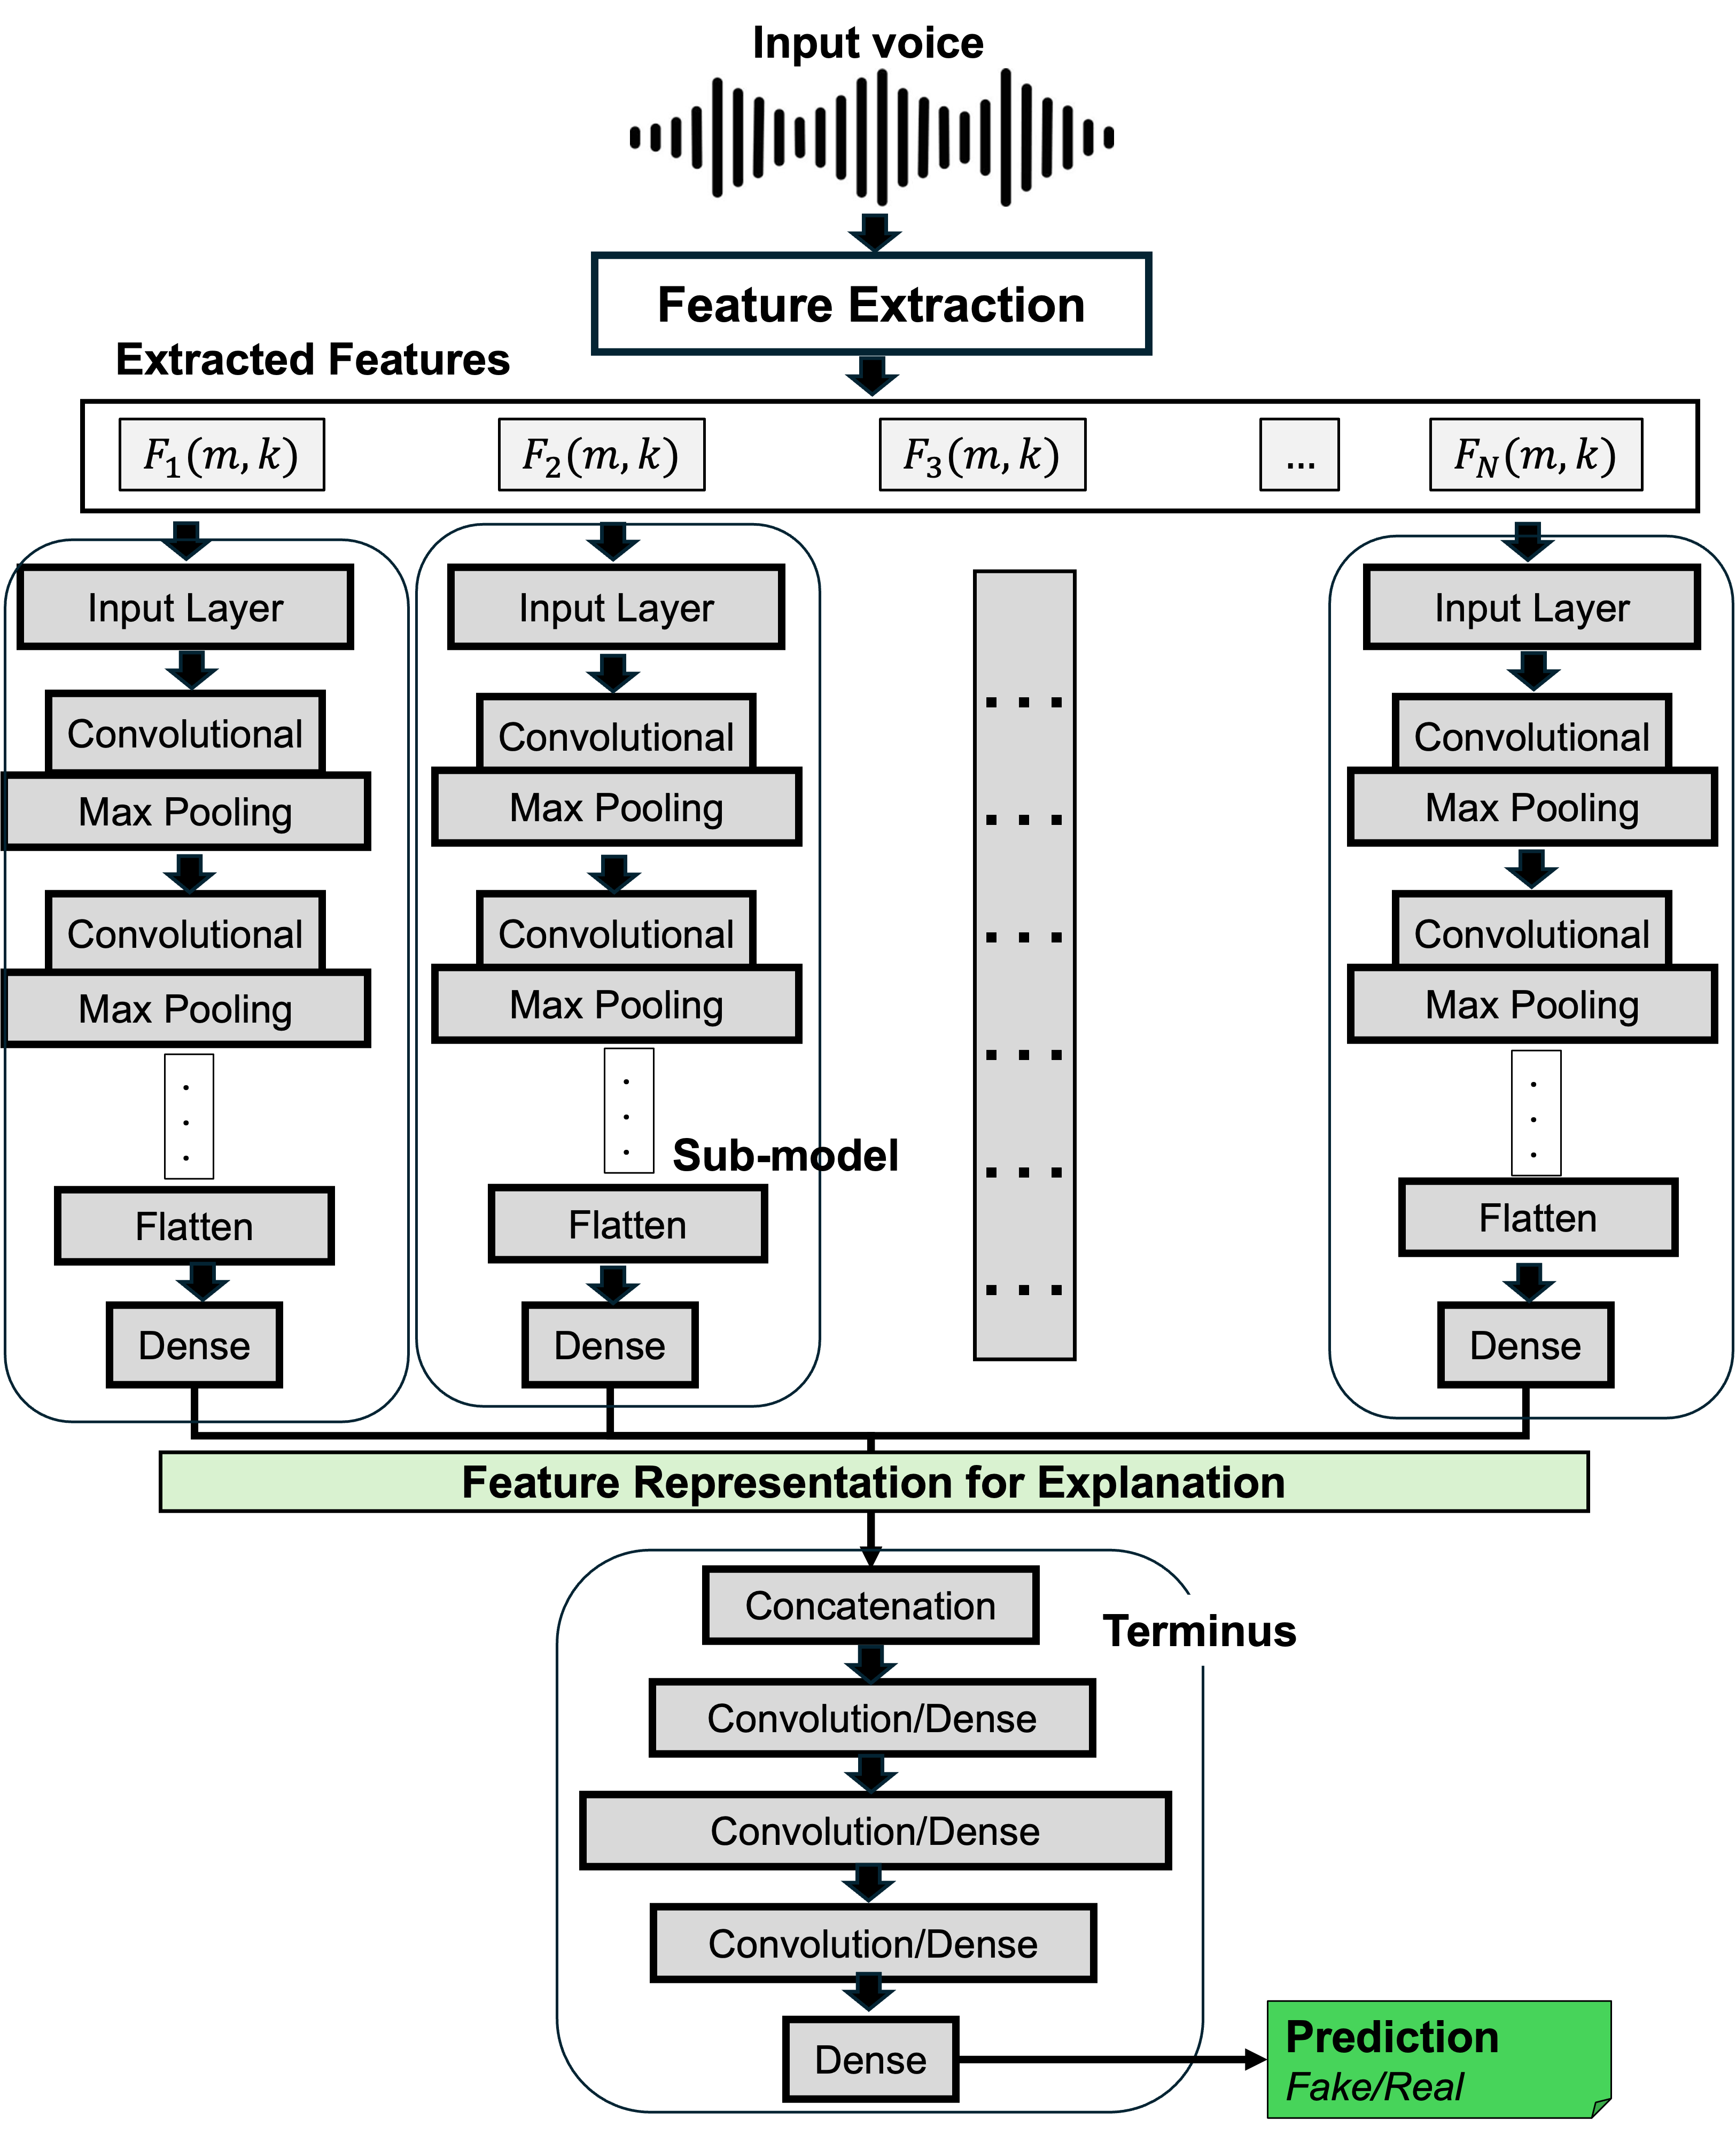
\includegraphics[width=0.75\linewidth]{images/Picture1.png}
    \caption{A high level building-block of our proposed hybrid fake voice identification model, where \(m\) and \(k\) represent the dimensionality of the given input feature.}
    \label{fig:overview}
\end{figure}
\section{Method}\label{sec:method}
Our proposed fake voice identification method consists of three major components including feature extractor, hybrid detection model, and the generation of explanations by modified LIME. After extracting features, we pass them individually through sub-models to overcome the multidimensionality problem. Then the concatenation of the outputs from the output layers of the sub-models are then passed through the \textit{terminus} models. For generating explanations, we make use of the feature values returned from the output layers of the sub-models, which has same representation of every feature. 

The high-level buidling-blocks of our hybrid interpretable deep fake voice identification model are presented in Fig.~\ref{fig:overview}. The architecture is more thoroughly discussed in Section \ref{sec:method_arch}.

\subsection{Feature Extraction}
The extracted features from audio samples can be categorized into two different classes: perceptible and imperceptible features. The perceptible features are features that can be perceived by the human ear, often vocal qualities such as jitter, shimmer or pitch fluctuation that have a wide range of uses even outside of audio classification such as diagnosis of disease~\cite{chaiwongyen_deepfake-speech_2023}, while imperceptible features are typically out of the range of human hearing, and may not directly reflect a vocal quality, otherwise referred to as ``speaker-independent'' features~\cite{liu_hidden--wave_2023}. In order to increase the likelihood that the explanations are useful and understandable to the end user, we focused on using multiple perceptible features as input to the classifier. However, we used two imperceptible features with the hypothesis, based on previous research~\cite{barrington_single_2023,chaiwongyen_contribution_2022,chaiwongyen_deepfake-speech_2023,li_comparative_2022}, that they would positively increase model performance. We extracted the following perceptible features:

\begin{itemize}
\item \textbf{Harmonic-to-noise ratios (HNRs)}: Inspired by previous research~\cite{chaiwongyen_contribution_2022,chaiwongyen_deepfake-speech_2023,		li_comparative_2022}, we extracted this features in a sliding window fashion instead of on the whole file. The HNRs are the ratios of the strengths of harmonic frequencies to the strengths of "noise" and the total strength outside the harmonic frequencies. Unlike previous research~\cite{chaiwongyen_contribution_2022, chaiwongyen_deepfake-speech_2023}, we computed this ratio for each fundamental frequency length, instead of using one value for the whole sample. Given that \(\gamma_{i}\) is the harmonic	energy in a given fundamental frequency cycle and \(\iota_{i}\) is the residual energy in a given fundamental frequency cycle, the HNR at that cycle \(hnr_{i}\) is calculated as follows:

\begin{equation}
    hnr_{i} = 20log\frac{\gamma_{i}}{\iota_{i}}.
\end{equation}

					

\item \textbf{Fundamental frequency lengths}: The fundamental frequency lengths, f0 length, are the lengths of every fundamental frequency cycle in the sample. This has also been previously employed and found effective in synthetic audio detection~\cite{xue_audio_2022}. The output is one-dimensional with time as the axis.

\item \textbf{Onset strength}: This perceptible feature represents the strengths of each onset in the audio sample, where an onset is point where there is a sudden rise in energy across the audio spectrum~\cite{li_comparative_2022}. This results in a one-dimensional output with time as the axis.

\item \textbf{Intensity}: Intensity is the total power at each point in the audio sample, given in \textit{db}. This is calculated by creating a Fourrier transformation of the sample and then summing across the frequency-axis for every point on the time-axis. Resulting in a one-dimensional output~\cite{li_comparative_2022}.

\item \textbf{Pitch-fluctuations}: The pitch fluctuations are calculated for every sample in the audio as the difference between pitch at the given point and the pitch at the previous point. Pitch is estimated based on the maximum power harmonics. This feature is similar to the use of summarized pitch fluctuations in previous research~\cite{khanjani_learning_2023}. This feature is also one-dimensional with time as the axis. Given that \(H_{i}\) is the set of harmonic frequencies at fundamental frequency cycle \(i\) with \(h_{i} \in H_{i}\) as a frequency of the set and \(s(h_{i})\) is the power of a given harmonic frequency at cycle \(i\), the pitch can be estimated as follows:
					                    
\begin{equation}
    p_{i} = s(max(H_{i})).
\end{equation}

Given an offset \(x\), the pitch fluctuation at cycle \(i\), \(pf_{i}\), can be calculated as follows:

\begin{equation}
    pf_{i} = p_{i}-p_{i-x}.
\end{equation}
   
\item \textbf{Jitter features}: Jitter~\cite{chaiwongyen_deepfake-speech_2023} measures the absolute variations in fundamental frequency cycles in comparison to the nearest \(x\) Neighbors. The jitter of a sample in relation to the nearest \(x\) samples can be described as follows:
\begin{equation}
    jitter(x) = \frac{ \frac{1}{N-1}\sum_{i=1}^{N-1}|T_{i}
						(\frac{1}{x}\sum_{n=i-m}^{i+m}T_{n})|}
					{\frac{1}{N}\sum_{i=1}^{N}T_{i}}, 
\end{equation}
					
where \(T_{i}\) represents the extracted fundamental frequency length at cycle \(i\), \(N\) is the number of fundamental frequency periods and \(m\) is \(\lfloor \frac{x}{2} \rfloor\).

\item \textbf{Shimmer features}: Similar to Jitter, shimmer instead make use of the amplitudes at each fundamental frequency period. The purpose is to capture irregular vocal fold vibrations which may be an indication but not a guarantee of a synthetic voice. The shimmer of a sample in comparison to the nearest \(x\) fundamental frequency cycles is calculated as follows~\cite{chaiwongyen_deepfake-speech_2023}:
\begin{equation}
    shimmer(x) = \frac{ \frac{1}{N-1}\sum_{i=1}^{N-1}|A_{i}
						(\frac{1}{x}\sum_{n=i-m}^{i+m}A_{n})|}
					{\frac{1}{N}\sum_{i=1}^{N}A_{i}},
\end{equation}
where \(A_{i}\) is the amplitude at cycle \(i\), \(N\) is the number of fundamental frequency cycles in the sample and \(m\) is once again \(\lfloor \frac{x}{2} \rfloor\)
			
\end{itemize}


We also chose to include two imperceptible features in our hybrid model, due to the performance-enhancing impact combining with the perceptible features~\cite{chaiwongyen_deepfake-speech_2023}. These features are the mel-spectrogram and their derivative mel-frequency cepstral coefficients. We select these two features as they are well established in the research and have demonstrated consistent high performance in existing state-of-the-art research~\cite{qais_deepfake_2022,anagha_audio_2023,fathan_mel-spectrogram_2022,altalahin_unmasking_2023,hamza_deepfake_2022,yan_initial_2022}. They allow for a	spectrographic representation and analysis of an audio sample transformed in a way to better represent human perception of frequencies~\cite{qais_deepfake_2022}.

\subsection{Hybrid Fake Voice Detection Model} \label{sec:method_arch}

Fig.~\ref{fig:overview} depicts the overall architecture of our hybrid deep learning model for fake voice identification. We propose an architecture for our hybrid fake voice detection model that allows for a combined classification based on features of different dimensionality, or in other words, regardless of whether the individual features have the same shape. To achieve this, we hypothesize that we can make use of individual separate models for each feature, which we will further refer to as \textit{sub-models}. The main objective for having the individual sub-models is to have similar representation of the features so that we can use them for generating understandable explanations. The structure of sub-model can be different based the dimension of the extracted features. For example, the dimension of convolution layers and max pooling layer would be different based on the dimension of the features. Sub-models may also omit the pooling layers all-together, as depicted in the example in Fig.~\ref{fig:alt_model_arch} (a), in order to have a structure based purely on convolution. We hypothesize that the use of convolution within these sub-models will increase the localized pattern detection capability of our method.

After the processing within the sub-models, we then needed to further process and distill the results into a singular output. To achieve this, followed by the concatenations of the output of all sub-models, we propose a terminus model. With the goal of maximizing performance, we tried various structures for the terminus models including single layer perceptron, convolutional neural networks and multi-layer perceptron. The figure (Fig.~\ref{fig:overview}) portrays a multi-layer terminus containing either convolutional layers hidden perceptron layers. However, a single perceptron layers is also possible and would look like a single dense layer after the flattened concatenation, as exemplified in Fig.~\ref{fig:alt_model_arch} (b). We discuss in the experiments section about our experimental settings.

\begin{figure}[htbp]
	\centering
    \subfloat[]{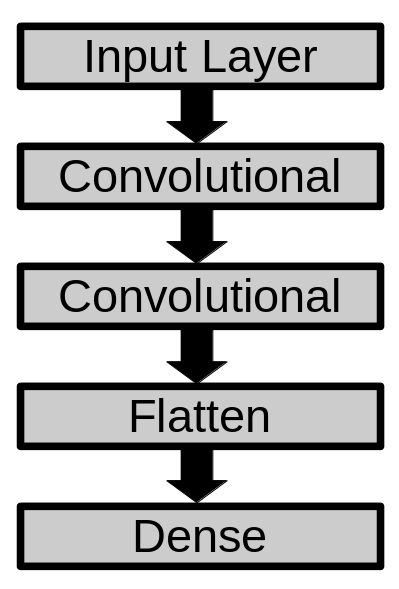
\includegraphics[width=0.25\textwidth]{images/alt_sub_model.png}} 
	\hfil
    \subfloat[]{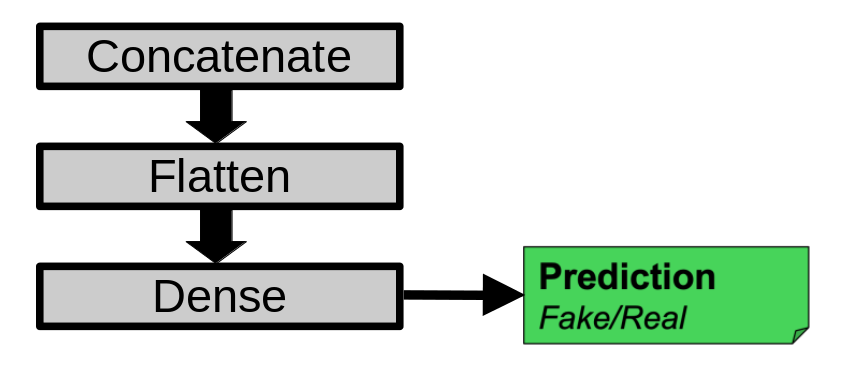
\includegraphics[width=0.5\textwidth]{images/simple_term.png}} 
	\caption{More examples for sub-model and terminus architectures, that deviate from the examples in Figure~\ref{fig:overview}. a) An example of a possible architecture of a sub-model without the inclusion of pooling layers. b) A terminus model with a simple perceptron architecture.}
    \label{fig:alt_model_arch}
\end{figure}

\subsection{Explaining the prediction}		\label{sec:method_exp}
		
We generate the explanations by creating an explainer with the Local Interpretable Model-agnostic Explanation (LIME) method~\cite{ribeiro_why_2016} using the previously described model as a surrogate. This section will describe in detail how individual explanations are generated at a local level for individual samples, as well as how we evaluate the usefulness of the explanations at a global scale.

\subsubsection{Generation of the Explanations}
Because of the multi-shaped nature and independence of the input layers of the model, we cannot generate the explanations directly from the input itself. However, being that the sub-models are separate from one another, having no influence on each other before being concatenated at the terminus, only the terminus part of the model is relevant for assessing the importance of the features in a single evaluation. Therefore, we make use of the processed features' values after the output layers of individual sub-models. This does, however, poses two challenges: i) there are multiple input rows per sample because a sliding-window is used across each audio sample and ii) the features cannot be used directly for assessment at the terminus input layer.

We solved the first problem by taking the mean of the weights returned by the LIME explainer of each feature produced by each row of the sample features. This results in an average contribution of each feature to the classification of the model. This is due to the fact that the end-classification of the surrogate is also a mean. Therefore, the averages of the weights from the LIME explainer represent aggregated influences of the features.

In order to address the second problem, we needed to, for each input feature, figure out what the output of the respective sub-model would be. This would allow us to transform the input into the one-dimensional input for the terminus model from the given sample in the input layers in every sub-model. After the processing of the sub-model, we catch the representation before the processing of the terminus model, which are one-dimensional similar representations of the features. This allows us to use the explainer to find a weight of each input of the terminus model in relation to the end result, prediction. We generate the sub-model results for a random sample of the training set to use as a reference for the localized model approximations from the LIME explainer.

We then summarized the results of the LIME explainer together on a per-feature basis and normalized them to produce a decimal number between -1 and 1 for every feature. In this case, a negative value implies that the given feature pushed the result of the model in the negative direction (i.e. not fake), while a positive value indicates the opposite.
			
            
\subsubsection{Evaluation of the Explanations}
In order to make an assessment the potential of this method of generating explanations, we needed a way to measure the influence of each feature on the average explanation generated using this method. In other words, we needed a method to assess the aggregated results of many explanations. Other methods such as SHAP (SHapley Additive exPlanations) \cite{lundberg2017unified} offer ways to explain features on a global scale, but due to their differing methodology in comparison with LIME, we see aggregated evaluations of a large number of local explanations as the best way to represent and assess the usefulness of our method. However, due to the lack of existing metrics for this purpose, we propose two new metrics with the intent of aggregate evaluation features present within local explanations.

In order to contextualize the metrics, we will make the following definitions.
    \begin{itemize}
        \item Let \(S\) be the set of samples with \(s \in S\) as an element of the set.
        \item Let \(F\) be the set of features with \(f \in F\) as an element of the set.
        \item Let \(w_{fs}\) be the weight value of feature \(f\) of sample \(s\) as
            produced by the explainer.
        \item Let \(l_{s}\) be the correct label of the sample \(s\).
    \end{itemize}
The first metric we propose is the mean of the absolute values of the weights of each feature within a set of explanations.
We will further refer to this metric as importance, and we define it mathematically as follows for every feature \(f \in F\) extracted from sample \(s \in S\):
\begin{equation}
    Imp(f, s) = \frac{\sum_{s \in S} |w_{fs}|}{|S|}.
\end{equation}
			
The second metric we will define is the average aggregate correctness on a per-feature basis, which we will further refer to as trust. The trust per feature \(f \in F\) extracted from sample \(s \in S \) can be defined as follows:
\begin{equation}
    Trust(f, s) = \frac{\sum_{s \in S} w_{fs}(2l_{s}-1)}{|S|}.
\end{equation}
			
            
\section{Experimental Results and Evaluation} \label{sec:experimental_results}
We carried out a wide range of experiments to validate the performance of our proposed interpretable hybrid fake voice identification model. The reminder of this section present the dataset that we used, experimental settings, experimental results, comparison with existing feature based models, the generated explanations and their evaluation.

\subsection{Dataset}
We trained and tested out model employing \textit{In-the-Wild} dataset. This dataset focuses on the generalization of audio deepfake detection models by collecting real-world data, in comparison to other research that used more controlled laboratory conditions~\cite{muller_does_2022}. We have chosen it for these experiments because of the aforementioned focus on generalization, its relative recency compared to some others and the fact that it has also been used previously by some other experiments, which provides a useful perspective against which we can compare our method.

The dataset consists of a total of 37.9 hours of audio samples, labelled as either bona-fide or fake. Of the total samples, 17.2 hours are fake while 20.7 hours are bona-fide audio. The fake samples were collected from online, publicly available video and audio clips that were specifically advertised as being deepfake clips. The bona-fide clips were then manually collected from genuine instances of the same speakers speaking from sources such as podcasts, speeches and so on. The clips were then segmented and downscaled to 16,000hz for the dataset.

\subsubsection{Training and Evaluation}
We trained the black-box model described in the previous section on the first portion of the dataset -- differing depending on the experiment -- and tested the models with the rest of the samples. Training batches consist of 100 samples each with every window position for each sample and an upper limit of 1,000,000 lines per batch, after which the batch will be further split. For each batch, either one or two epochs were performed. Because a single sample can have multiple input lines, evaluation cannot be performed on a per-line basis, but must instead be summarized. Two methods are possible: median and mean, with the difference in results being negligible in our experiments. The default threshold is 0.5, meaning that a result under 0.5 is a negative result and over 0.5 is a positive result. This threshold can however be adjusted, useful for computing certain metrics. We compute the model performance by employing equal error rate (ERR) metric. The lower the value of ERR, the better the performance of the model is. However, we have different experimental settings based on the structure of terminus model, features applied and number samples to train the models. In addition to the label, the samples are also annotated with the given speaker.

\subsection{Results}
We present experimental results for all variations of our proposed model in Table~\ref{table:eval-results}. The table details the following information: The type of terminus model used, where ``perceptron'' does not include hidden layers, MPL(3) is a multi-perceptron layer model with three hidden layers and CNN (3) is a convolutional neural network with three hidden layers; we used different set of features, where ``standard'' is the feature set as described above including only one pitch-fluctuation feature. However, with expanded pitch fluctuations, we combine the same feature set with the addition of more pitch fluctuation features with different comparison distances; the training batch size and the number of epochs per batch if there were more than one; followed by several performance metrics. 

\begin{table}[htbp]
			\caption{Summary of the evaluation results of the experiments}
			\vspace{10pt}
			\centering
			\footnotesize
			\begin{tabular}{|c | c | c | c | c | c|}
				\hline
				\textbf{Terminus} & \textbf{Features} & \textbf{Training} & \textbf{Accuracy} & \textbf{EER} & \textbf{AUC} \\
				\hline 
				Perceptron & standard & 3474 & 95.02\% & 0.03702 & 0.90297 \\ \hline
				MPL (3) & standard & 10000 & \textbf{96.27\%} & \textbf{0.03214} & 0.81763 \\ \hline
				Perceptron & standard & 23833 2 epochs & 90.07\% & 0.90069 & 0.78889 \\ \hline
				Perceptron & standard & 10000 2 epochs & 94.43\% & 0.04408 & 0.89445 \\ \hline
				Perceptron & standard & 10000 & 94.28\% & 0.04840 & 0.90182 \\ \hline
				CNN (3) & standard & 10000 & 62.80\% & 0.37198 & 0.50051 \\ \hline
				Perceptron & expand pitch\-flucs & 10000 & 93.31\% & 0.05661 & \textbf{0.92727} \\ \hline
				MPL (3) & expand pitch\-flucs & 10000 & 93.87\% & 0.05317 & 0.83263 \\ \hline
			\end{tabular}
			\label{table:eval-results}
		\end{table}

We can see that the hybrid model with an MLP terminus model trained with standard features set on first 100000 samples achieved higher accuracy (96.27\%) and ERR (0.03214). However, the model with perceptron as a terminus applying features with expanded pitch fluctuations-based features performed better than other experimental settings in terms of AUC (0.92727). The other experimental settings also performed comparatively except with terminus models based on convolutional neural networks. Percepton-based terminus models with all variation also performed effectively with (2-3)\% deviation compared to best performing model.


\begin{figure}
    \centering
    \subfloat[]{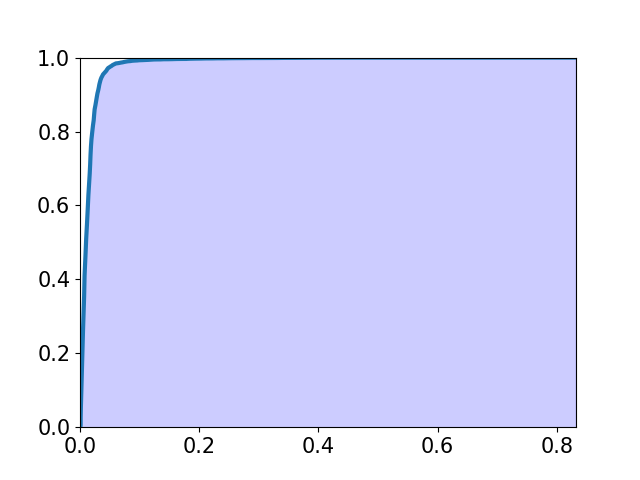
\includegraphics[width=0.27\textwidth]{images/roc_cterm.png}} 
    \subfloat[]{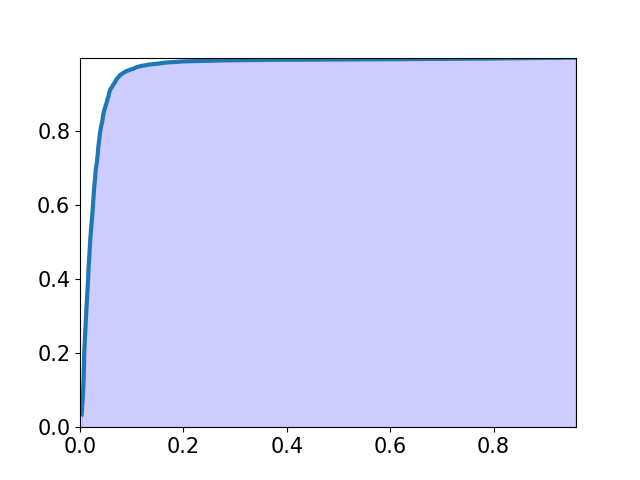
\includegraphics[width=0.27\textwidth]{images/roc_mpf.png}} 
    \subfloat[]{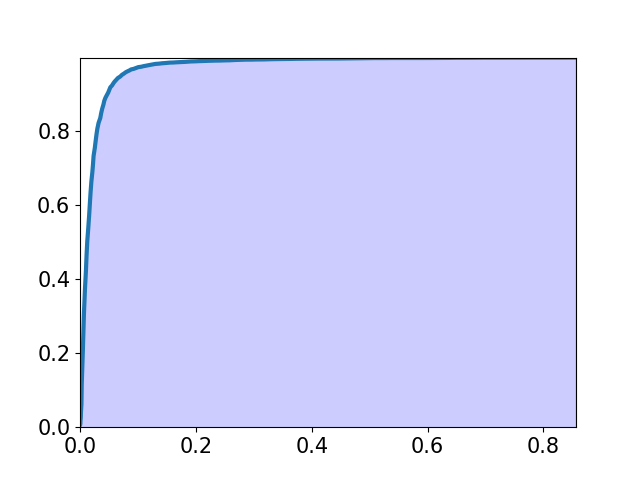
\includegraphics[width=0.27\textwidth]{images/roc_mpf_cterm.png}}
    \caption{ROC Curves. a) ROC for best performing model, b) ROC curve for the model with pitch fluctuation features and c) ROC curve for the model with MLP-based terminus and expanded pitch fluctuation features.}
    \label{ROC_curves}
\end{figure}

Figure~\ref{ROC_curves} depicts the ROC curves for three of the models, which were selected for use in explanation generation in Section \ref{sec:method_metrics}.

\subsubsection{Comparison with Existing Methods}
\begin{table}
    \caption{Performance comparison of our method with existing methods applied on the same dataset.}
    \vspace{10pt}
    \centering
    \begin{tabular}{|c|c | c|}
        \hline
        \textbf{Author} & \textbf{Methods} & \textbf{Equal Error Rate (ERR)} \\ \hline
        Ranjan et al.\cite{ranjan_statnet_2022} & STATNet  & \textbf{0.00199} \\ \hline
        Our Method &\textbf{Hybrid DL} & 0.03214 \\  \hline
        \multirow{3}{*}{Yang et al.~\cite{yang_robust_2024}} &	Fusion & 0.2427 \\ \cline{2-3}
        &	Selection  & 0.2598 \\ \cline{2-3}
        &	ResNet18  & 0.2748 \\ \hline
        
        \multirow{3}{*}{Yi et al.~\cite{yi_audio_2023}}    &	ASSERT  & 0.2473 \\ \cline{2-3}
        &	LCNN  & 0.3514 \\ \cline{2-3}
        &	GMM & 0.3749 \\ \hline

        \multirow{12}{*}{Müller et al.~\cite{muller_does_2022}} 
        &	RawGAT-ST \cite{muller_does_2022} & 0.37154 \\ \cline{2-3}
        &	MesoInception \cite{muller_does_2022} & 0.37414 \\ \cline{2-3}        
        &	RawNet2  & 0.37819 \\ \cline{2-3}
        &	Transformer  & 0.43775 \\ \cline{2-3}
        &	CRNNSpoof & 0.44500 \\ \cline{2-3}
        &	RawPC  & 0.45715 \\ \cline{2-3}
        &	MesoNet & 0.46939 \\ \cline{2-3}
        &	ResNet18  & 0.49759 \\ \cline{2-3}
        &	LSTM  & 0.53711 \\ \cline{2-3}
        &	LCNN-LSTM  & 0.61500 \\ \cline{2-3}
        &	LCNN  & 0.65559 \\ \cline{2-3}
        &	LCNN-Attention  & 0.66684 \\ \hline
    \end{tabular}
    \label{table:other_results}
\end{table}
In order to contextualize our results, we compare them to other results produced using tests on the same dataset. Table \ref{table:other_results} presents some experimental results that other methods have achieved on this dataset, sorted by source and model architecture. When multiple experiments with one method were done, the best result was used for this table. The results only include evaluations on the full length samples, and not cropped versions, as we tested on the full-length samples. The performances are compared in terms of EER, and the best result is in bold. In comparison to the other methods, our method outperformed all other existing methods excepts one by Ranjan et al.~\cite{ranjan_statnet_2022}. Their method used an expanded RawNet2-based network, taking the raw waveform as an input. They trained their method on 70\% of the dataset, used 10\% for validation and the remaining 20\% for testing. This indicates a potential for raw-waveform based learned feature in the accurate detection of audio deepfakes, but does not offer a clear path for explainability, as the model does not make any intrinsic distinction of audio characteristics that humans are able to perceive. On contrary, we leveraged only hand-crafter features and still our method is competitive, indicating that it can provide a good base for trustworthy explanations. Since we process every feature through individual sub-models, the out representation can capture better information about the feature and that might help in the concatenation to perform better classification performance in terminus model. To visualize the performance comparison better, we present the comparison as a bar chart in Fig.~\ref{comparison_bar}.

    \begin{figure}[htbp]
        \centering
        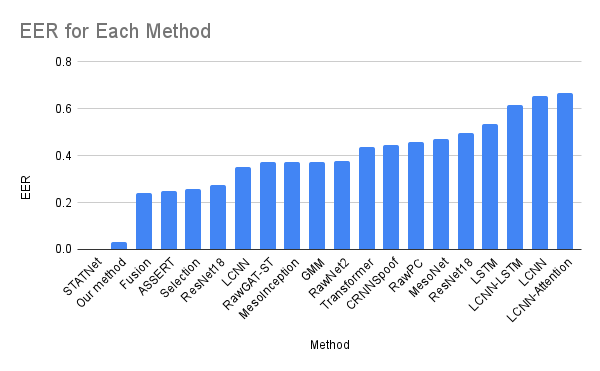
\includegraphics[width=0.95\textwidth]{images/method_comparison.png}
        \caption{A visual representation of the EER results of our method against some other methods from the literature. The lower the value of EER, the better the method is.}
        \label{comparison_bar}
    \end{figure}


            
\subsection{Evaluating explanations generated by LIME} \label{sec:method_metrics}
In order to obtain a comprehensive understanding of the quality of the explanations generated by LIME, we selected the three best-performing models and generated explanations for the first 500 samples of the testing data. These three models achieved the best performance in terms of Accuracy and Equal Error Rate (EER) or AUC. They include: a model using the standard feature set with a terminus model containing three hidden layers, model with expanded pitch-fluctuation features and a perceptron terminus, which achieved the best AUC result, and model with expanded pitch-fluctuation features and a terminus containing three hidden layers.

We selected these models to evaluate the best-performing configurations and to observe how the inclusion of expanded pitch-fluctuation features affects the evaluation of the explanations. We then aggregated and summarized the explanations using the two previously introduced metrics: trust and importance. A summary of the evaluation in terms of these metrics, grouped by feature, is presented in Tables~\ref{table:exp-results-cterm}, \ref{table:exp-results-more-pitch-flucs}, and \ref{table:exp-results-mpf-cterm}. The same statistics are also represented graphically in Figures \ref{fig:exp_cterm}, \ref{fig:exp_mpf}, and \ref{fig:exp_mpf_cterm}, respectively.
\begin{table}[htbp]
	\caption{Evaluation of generated explanations in terms of \textit{trust} and \textit{importance} for best performing model in terms of EER}
			\vspace{10pt}
			\centering
			\begin{tabular}{|c | c | c|}
				\hline
				\textbf{Feature} & \textbf{Importance} & \textbf{Trust} \\
				\hline
				HNRs & 0.1140 & -0.0543 \\  \hline
				mel spectrogram & 0.1084 & -0.0378 \\ \hline
				MFCC & \textbf{0.7029} & \textbf{0.3753} \\ \hline
				f0 lengths & 0.0 & 0.0 \\ \hline
				onset strengths & 0.0 & 0.0 \\ \hline
				intensities & 0.0 & 0.0 \\ \hline
				pitch fluctuations & 0.0 & 0.0 \\ \hline
				jitter features & 0.1277 & 0.0250 \\ \hline
				shimmer features & 0.1227 & 0.0017 \\ \hline
			\end{tabular}
			\label{table:exp-results-cterm}
		\end{table}
		
\subsubsection{Model with Standard Feature Set and MLP based Terminus}
According to both metrics, we can see that in Table~\ref{table:exp-results-cterm} and Fig.~\ref{fig:exp_cterm}, the MFCCs had the most positive and accurate influence on the classification results, with the jitter features being a distant second in terms of trust and importance. This indicates that the MFCCs not only had the greatest influence but also the most reliable impact on the classification outcomes. In contrast, other features had little, no, or even negative influence on the classification. However, the jitter features are notable as perceptible features with a positive trust value.
\begin{figure}
			\centering
			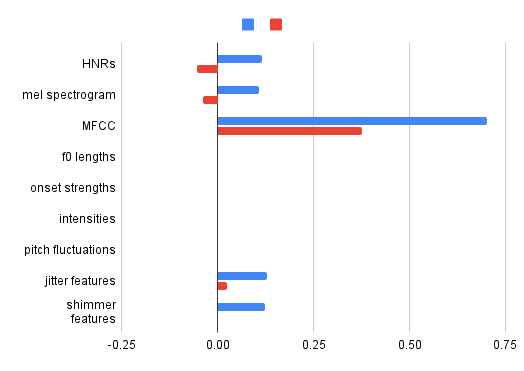
\includegraphics[width=0.7\textwidth]{images/exp_cterm.png}
			\caption{Graphical representation of the evaluation of generated explanations in terms of \textit{trust} and \textit{importance} for best performing model in terms of EER}
			\label{fig:exp_cterm}
		\end{figure}
        
\begin{table}[htbp]
			\caption{Evaluation of generated explanations in terms of \textit{trust} and \textit{importance} model with expanded pitch fluctuation features}
			\vspace{10pt}
			\centering
			\begin{tabular}{|c | c | c|}
				\hline
				\textbf{Feature} & \textbf{Importance} & \textbf{Trust} \\
				\hline
				HNRs & 0.1072 & -0.0148 \\ \hline
				mel spectrogram & 0.0428 & -0.0187 \\ \hline
				MFCC & \textbf{0.4383} & \textbf{0.2345} \\ \hline
				f0 lengths & 0.0340 & -0.0057 \\ \hline
				onset strengths & 0.0101 & -0.0027 \\ \hline
				intensities & 0.0021 & 0.0021 \\ \hline
				pitch fluctuations & 0.0059 & 0.0020 \\ \hline
				jitter features & 0.2439 & 0.0019 \\ \hline
				shimmer features & 0.1664 & 0.0070 \\ \hline
			\end{tabular}
			\label{table:exp-results-more-pitch-flucs}
		\end{table}	
\subsubsection{Model with Expanded Pitch-Fluctuation Features}
Table~\ref{table:exp-results-more-pitch-flucs} and Fig.~\ref{fig:exp_mpf} illustrate that this model produced comparable results, with the key difference being that all features had non-zero values for both metrics. This means that every feature influenced the classifications used to generate the explanations. Similar to the previous model, HNRs and mel-spectrograms had negative overall trust values, with the addition of onset strengths also showing a negative value. This implies that these features caused more harm than good in the tested classifications. Notably, both jitter and shimmer features had positive trust values, highlighting their potential as trustworthy perceptible features for explanations.

	\begin{figure}
			\centering
			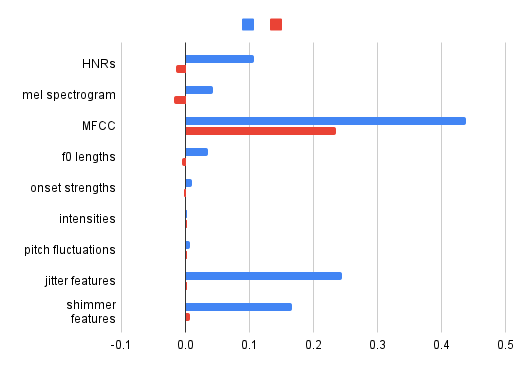
\includegraphics[width=0.7\textwidth]{images/exp_mpf.png}
			\caption{Graphical representation of the evaluation of generated explanations in terms of \textit{trust} and \textit{importance} model with expanded pitch fluctuation features.}
			\label{fig:exp_mpf}
		\end{figure}
\begin{table}[htbp]
			\caption{Evvaluation of generated explanations in terms of \textit{trust} and \textit{importance} for the model with expanded pitch fluctuation features and a terminus with MLP.}
			\vspace{10pt}
			\centering
			\begin{tabular}{|c | c | c|}
				\hline
				\textbf{Feature} & \textbf{Importance} & \textbf{Trust} \\
				\hline
				HNRs & 0.2667 & -0.0788 \\ \hline
				mel spectrogram & 0.0982 & -0.0434 \\ \hline
				MFCC & \textbf{0.2879} & \textbf{0.2408} \\ \hline
				f0 lengths & 0.1690 & -0.0521 \\ \hline
				onset strengths & 0.1384 & -0.0613 \\ \hline
				intensities & 0.1576 & -0.0504 \\ \hline
				pitch fluctuations & 0.0 & 0.0 \\ \hline
				jitter features & 0.1444 & 0.0118 \\ \hline
				shimmer features & 0.1747 & 0.0116 \\ \hline
			\end{tabular}
			\label{table:exp-results-mpf-cterm}
		\end{table}

\subsubsection{Model with Expanded Pitch-Fluctuation Features and MLP Terminus}
Table~\ref{table:exp-results-mpf-cterm} and Fig.~\ref{fig:exp_mpf_cterm} present the results for the evaluation of the explanations for the model with pitch fluctuation features and MLP terminus. The model combining multiple pitch-fluctuation features with a terminus containing multiple hidden layers performed similarly to the other two models. However, in this case, the pitch fluctuations had no influence on the outcomes. Unlike the previous examples, the intensities feature had a negative trust value. Nevertheless, the trust values for the jitter and shimmer features remained positive, reinforcing their reliability as perceptible features for generating meaningful explanations.
		\begin{figure}
			\centering
			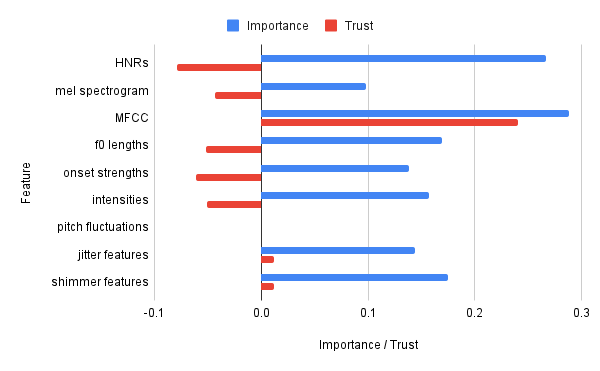
\includegraphics[width=0.7\textwidth]{images/exp_mpf_cterm.png}
			\caption{Graphical representation of the evaluation of generated explanations in terms of \textit{trust} and \textit{importance} for the model with expanded pitch fluctuation features and a terminus with MLP.}
			\label{fig:exp_mpf_cterm}
		\end{figure}

\section{Discussion}\label{sec:discussion}
In this section, we discuss the implications of the experimental results presented in the previous sections, with a special focus being placed on the evaluation of the generated explanations as it relates to the potential explainability for potential end users of such a system.
		
\subsection{Viability and Potential of the Explanations}

We hypothesized that explanations leveraging perceptible features have high potential to enhance the interpretability of complex ML model predictions. Moreover, perceptible features can present explanations in a more comprehensible manner for end users. However, as shown in the previous section in Tables \ref{table:exp-results-cterm} and \ref{table:exp-results-more-pitch-flucs}, perceptible features contributed less to classification performance than their imperceptible counterparts, despite their increased presence in the overall set of input features.

Two features—HNRs and mel-spectrograms—even consistently had a net-negative impact on classification accuracy in our experiments, as measured by our \textit{trust} metric. This leaves an open question as to whether future experiments might perform better without these features. In the model without expanded pitch fluctuations, four perceptible features—f0 lengths, onset strengths, intensities, and pitch fluctuations—had an overall average influence of zero on classification across both metrics. This suggests that the model did not learn a meaningful correlation between these features and the authenticity of audio samples in the dataset. Although these features did have some impact on the performance of the model with expanded pitch fluctuations, the effect remained minimal.

For perceptible features with a positive \textit{trust} score, there remains potential for their use in generating understandable explanations. Even though these features did not significantly influence the model’s predictions, they still demonstrate a certain level of reliability. Nevertheless, we believe it is worth investigating whether other types of perceptible features might exert a stronger influence on classification or whether alternative imperceptible features—potentially replacing MFCCs—could achieve a better balance between classification accuracy and proportional influence on the final result. This would enhance the usefulness of explanations beyond those produced using the current feature combinations. Furthermore, we believe that this model architecture, when paired with LIME and evaluated using the proposed metrics, has the potential to serve as a foundation for future research.

\subsection{Limitations}
Despite the potential of this method, it also presents certain limitations regarding real-world applicability, beyond the shortcomings of perceptible features discussed in the previous section. The first major limitation concerns computational performance. Due to its relative size, the model requires high-performance hardware and several gigabytes of memory to classify samples. As a result, the range of devices capable of running this or a similar model is restricted, and, at the time of writing, deploying it locally on a handheld device such as a smartphone is practically infeasible.

Another limitation of this method is that, while perceptible features like those used in our approach are known to be audible to the human ear and are even utilized in medical diagnoses~\cite{chaiwongyen_deepfake-speech_2023}, the extent to which these features are intuitively understandable to the average person remains unclear. Preliminary research~\cite{warren_better_2024,sharevski_blind_2024} has explored the factors humans use to differentiate real from fake audio samples and assessed their performance in doing so. However, these identified aspects have not yet been explicitly mapped to the perceptible features used in our method. This raises an open question regarding the usability of such explanations and whether additional perceptible features could be extracted to align more closely with the cues humans use to identify fake voice samples.

Finally, our experiments did not address how these features should be presented to end users. While certain implementations of LIME already offer graphical representations of their results, the effectiveness of such visualizations has yet to be systematically studied.

\section{Conclusion}
To conclude, we have presented a hybrid interpretable deep learning model that leverages a combination of heterogeneous features, both perceptible and imperceptible. We hypothesized that such a model could be used to generate explanations using LIME, which might be more useful for potential end users. The experimental results demonstrated top-tier performance in accurately identifying fake voices while mitigating the dimensionality problem in the input features. We observed that explanations leveraging the representations just before the model’s final layer can generate technical insights. These explanations might be useful for improving model performance by modifying important parameters or as the basis for presenting an analysis of a sample to an end user, in the case where perceptible features have an influence on the classification, so they can understand if audible flaws in the sample are present. However, based on our proposed metrics, \textit{trust} and \textit{importance}, we did not observe a significant influence or usefulness of perceptible features, although they did contribute to explanations to some extent.

A promising direction for future work would be integrating this method into different domains where feature-based local explanations have the potential to be effective. In such application domains, we could further validate both the accuracy and the usefulness of the generated explanations as well as the selected features using our proposed metrics. Additionally, it would be valuable to compare findings from a user study on the generated explanations with our metric-based evaluation.
	\newpage
	\sloppy
	\printbibliography
	\newpage
	\section{Erklärung}
	Hiermit versichere ich, dass ich die vorliegende Arbeit selbstständig, insbesondere auch nicht mit Hilfe einer KI-Software, angefertigt habe. Ich habe ausschließlich die angegebenen Hilfsmittel und Quellen benutzt; das betrifft auch Quellen und andere Informationen aus dem Internet. Alle Stellen, die wörtlich oder sinngemäß aus veröffentlichten und nicht veröffentlichten fremden Schriften entnommen wurden, sind als solche kenntlich gemacht.

	Die Paragraphen der für mich geltenden Prüfungsordnungen, die etwaige Betrugs-versuche betreffen, habe ich zur Kenntnis genommen.

	Der Speicherung meiner Abschlussarbeit zum Zweck der Plagiatsprüfung stimme ich zu. Ich versichere, dass die elektronische Version mit der gedruckten Version inhaltlich übereinstimmt. \\ \\ \\ \\ 
	\hline
	Datum \quad \quad \quad \quad \quad \quad \quad \quad Unterschrift
\end{document}
